\section{Field Trip and Open-Source Inspiration}
\label{app:field}
The author confirms attending both the Tencent Shanghai Office and Shanghai Science and Technology Museum on September 4, 2026 and personally taking both photographs. The files were copied unchanged from the author's v1 project. The images record visible displays, not evidence for the present game's equilibria or observed free-riding.

\subsection{Tencent Shanghai Office --- September 4, 2026}
\begin{center}
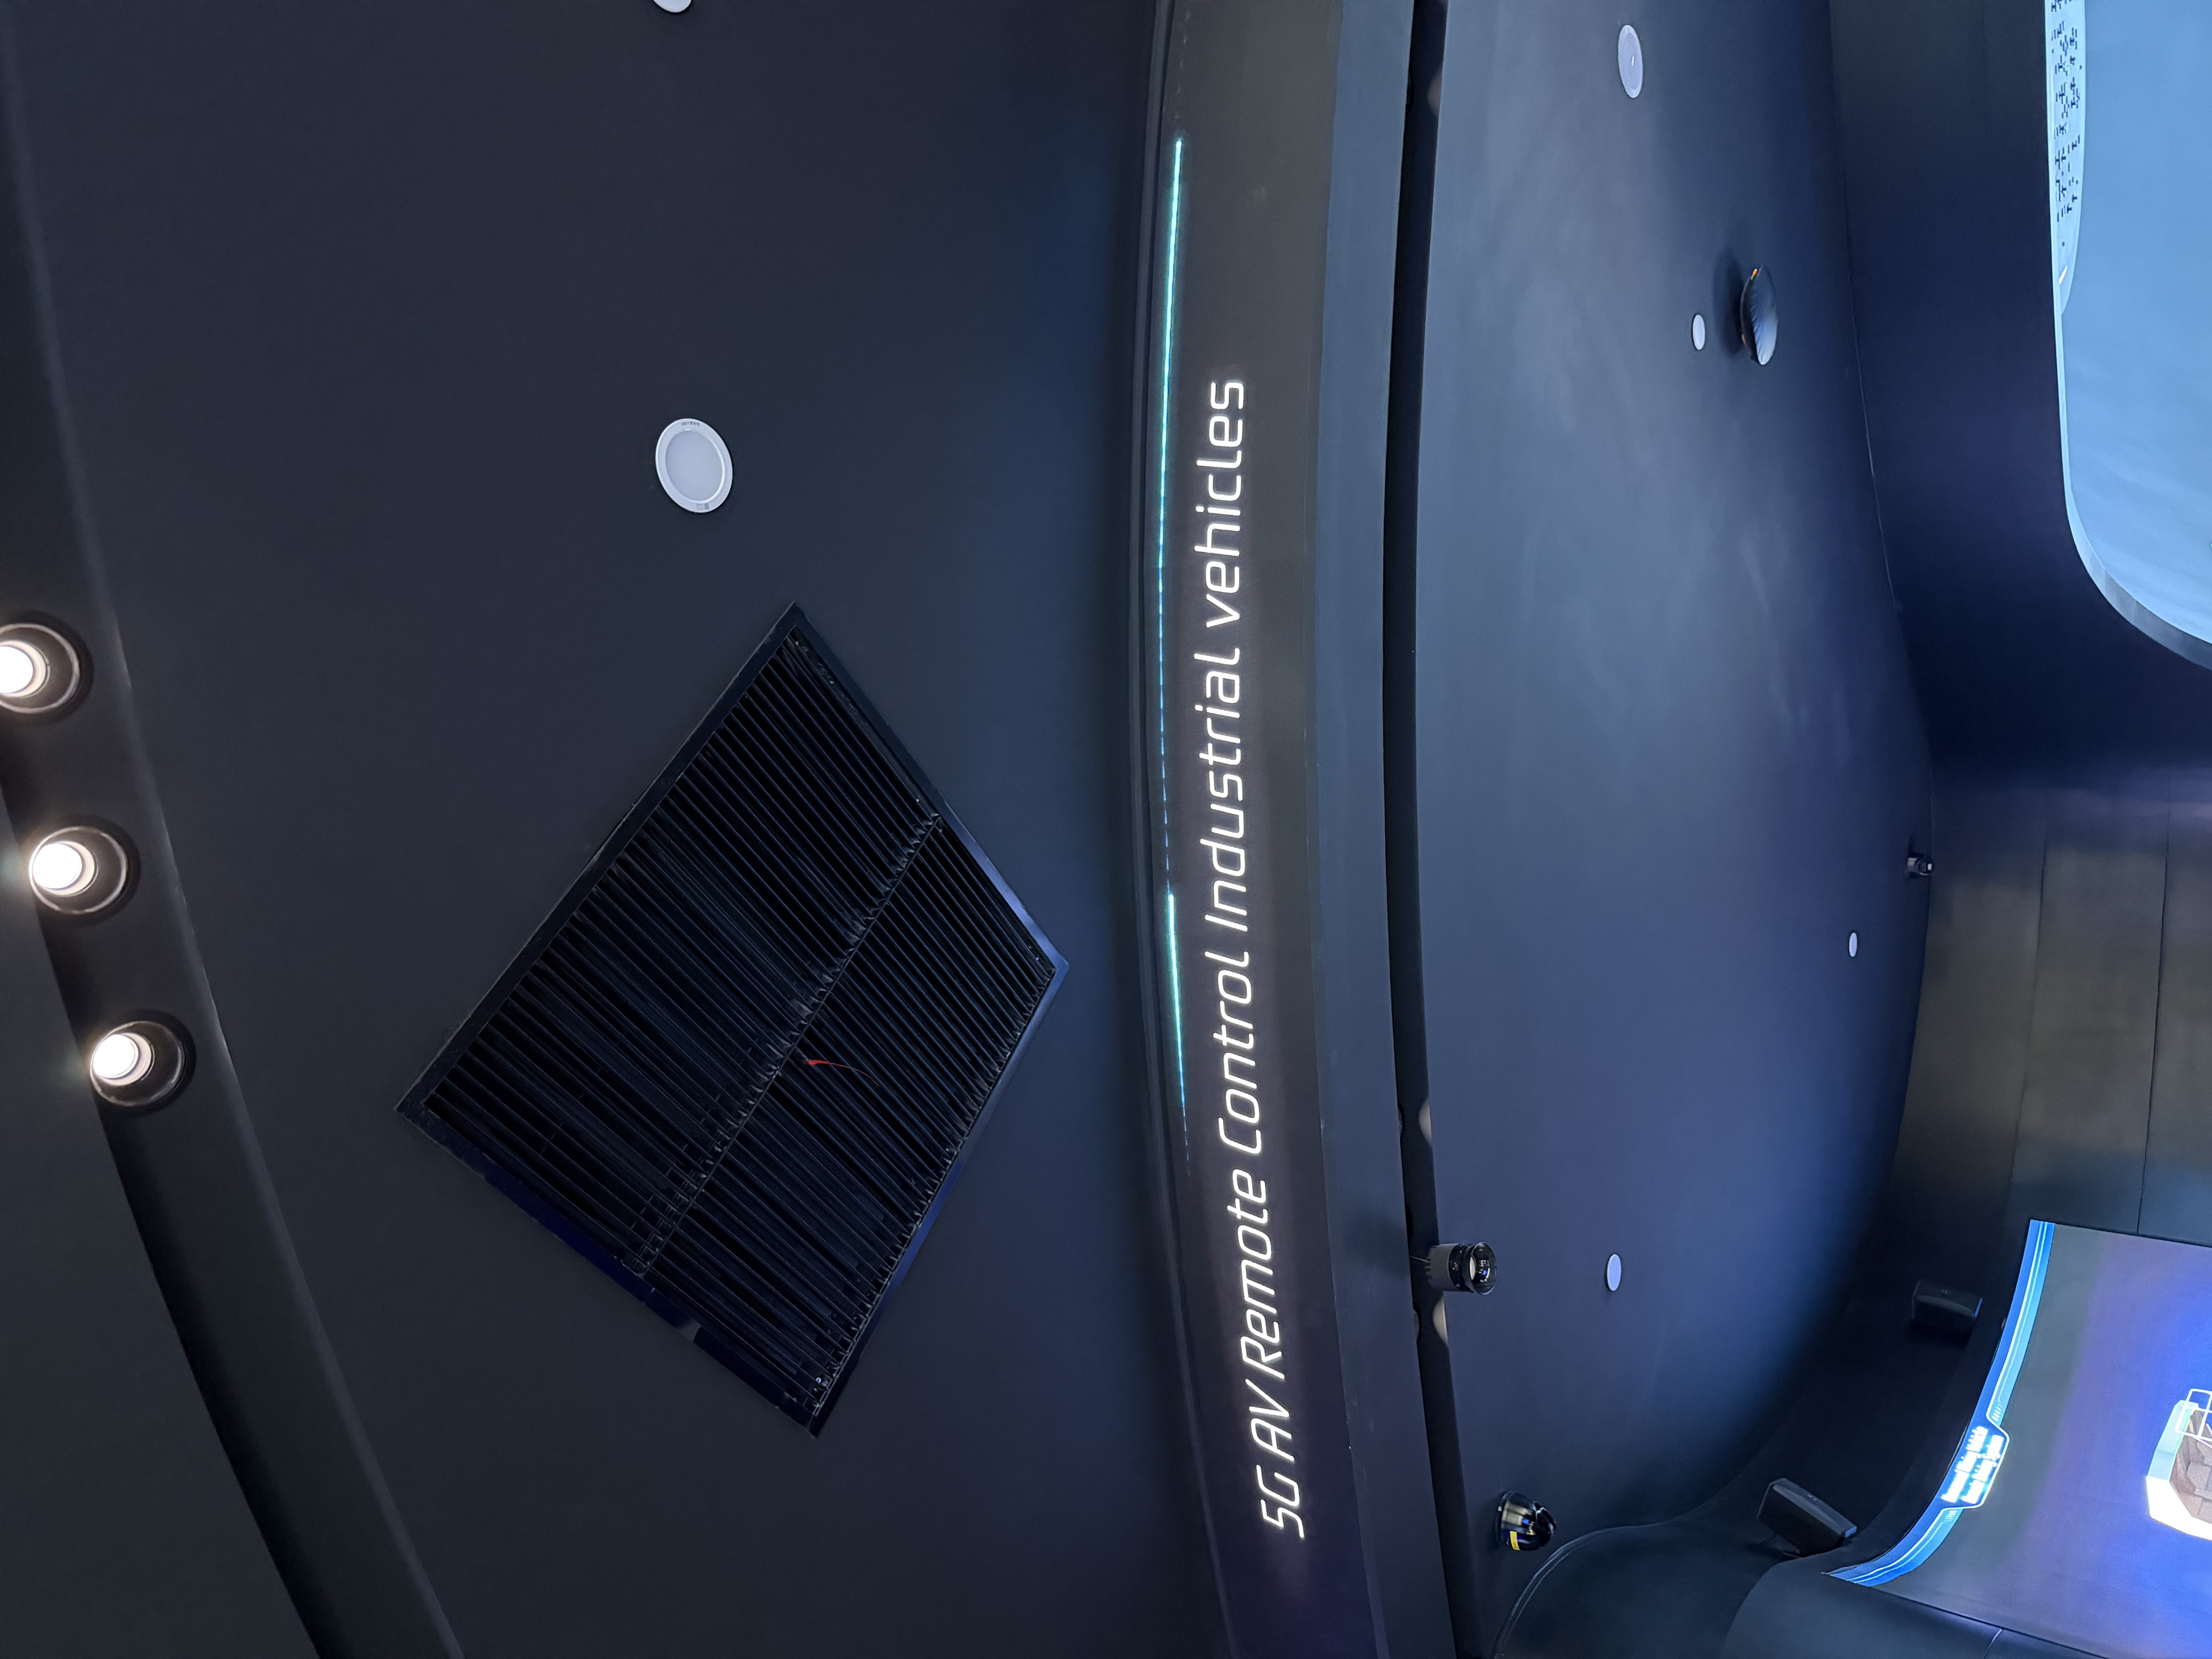
\includegraphics[width=0.55\linewidth,angle=-90]{field_trip/tencent_shanghai_office.jpg}
\end{center}
\noindent\textbf{Photograph caption:} Technology display at Tencent Shanghai Office with the visible heading ``5G AV Remote Control Industrial Vehicles.'' Photograph by Yiqiao Liu (Mickey), September 4, 2026.

\noindent\textbf{Observation:} The photograph shows an illuminated heading and part of a technology display. \textbf{Interpretation:} The visit exposed the author to practical automated systems and motivated broader questions about coordination and responsibility; the image does not show strategic information acquisition or a tested equilibrium.

\subsection{Shanghai Science and Technology Museum --- September 4, 2026}
\begin{center}
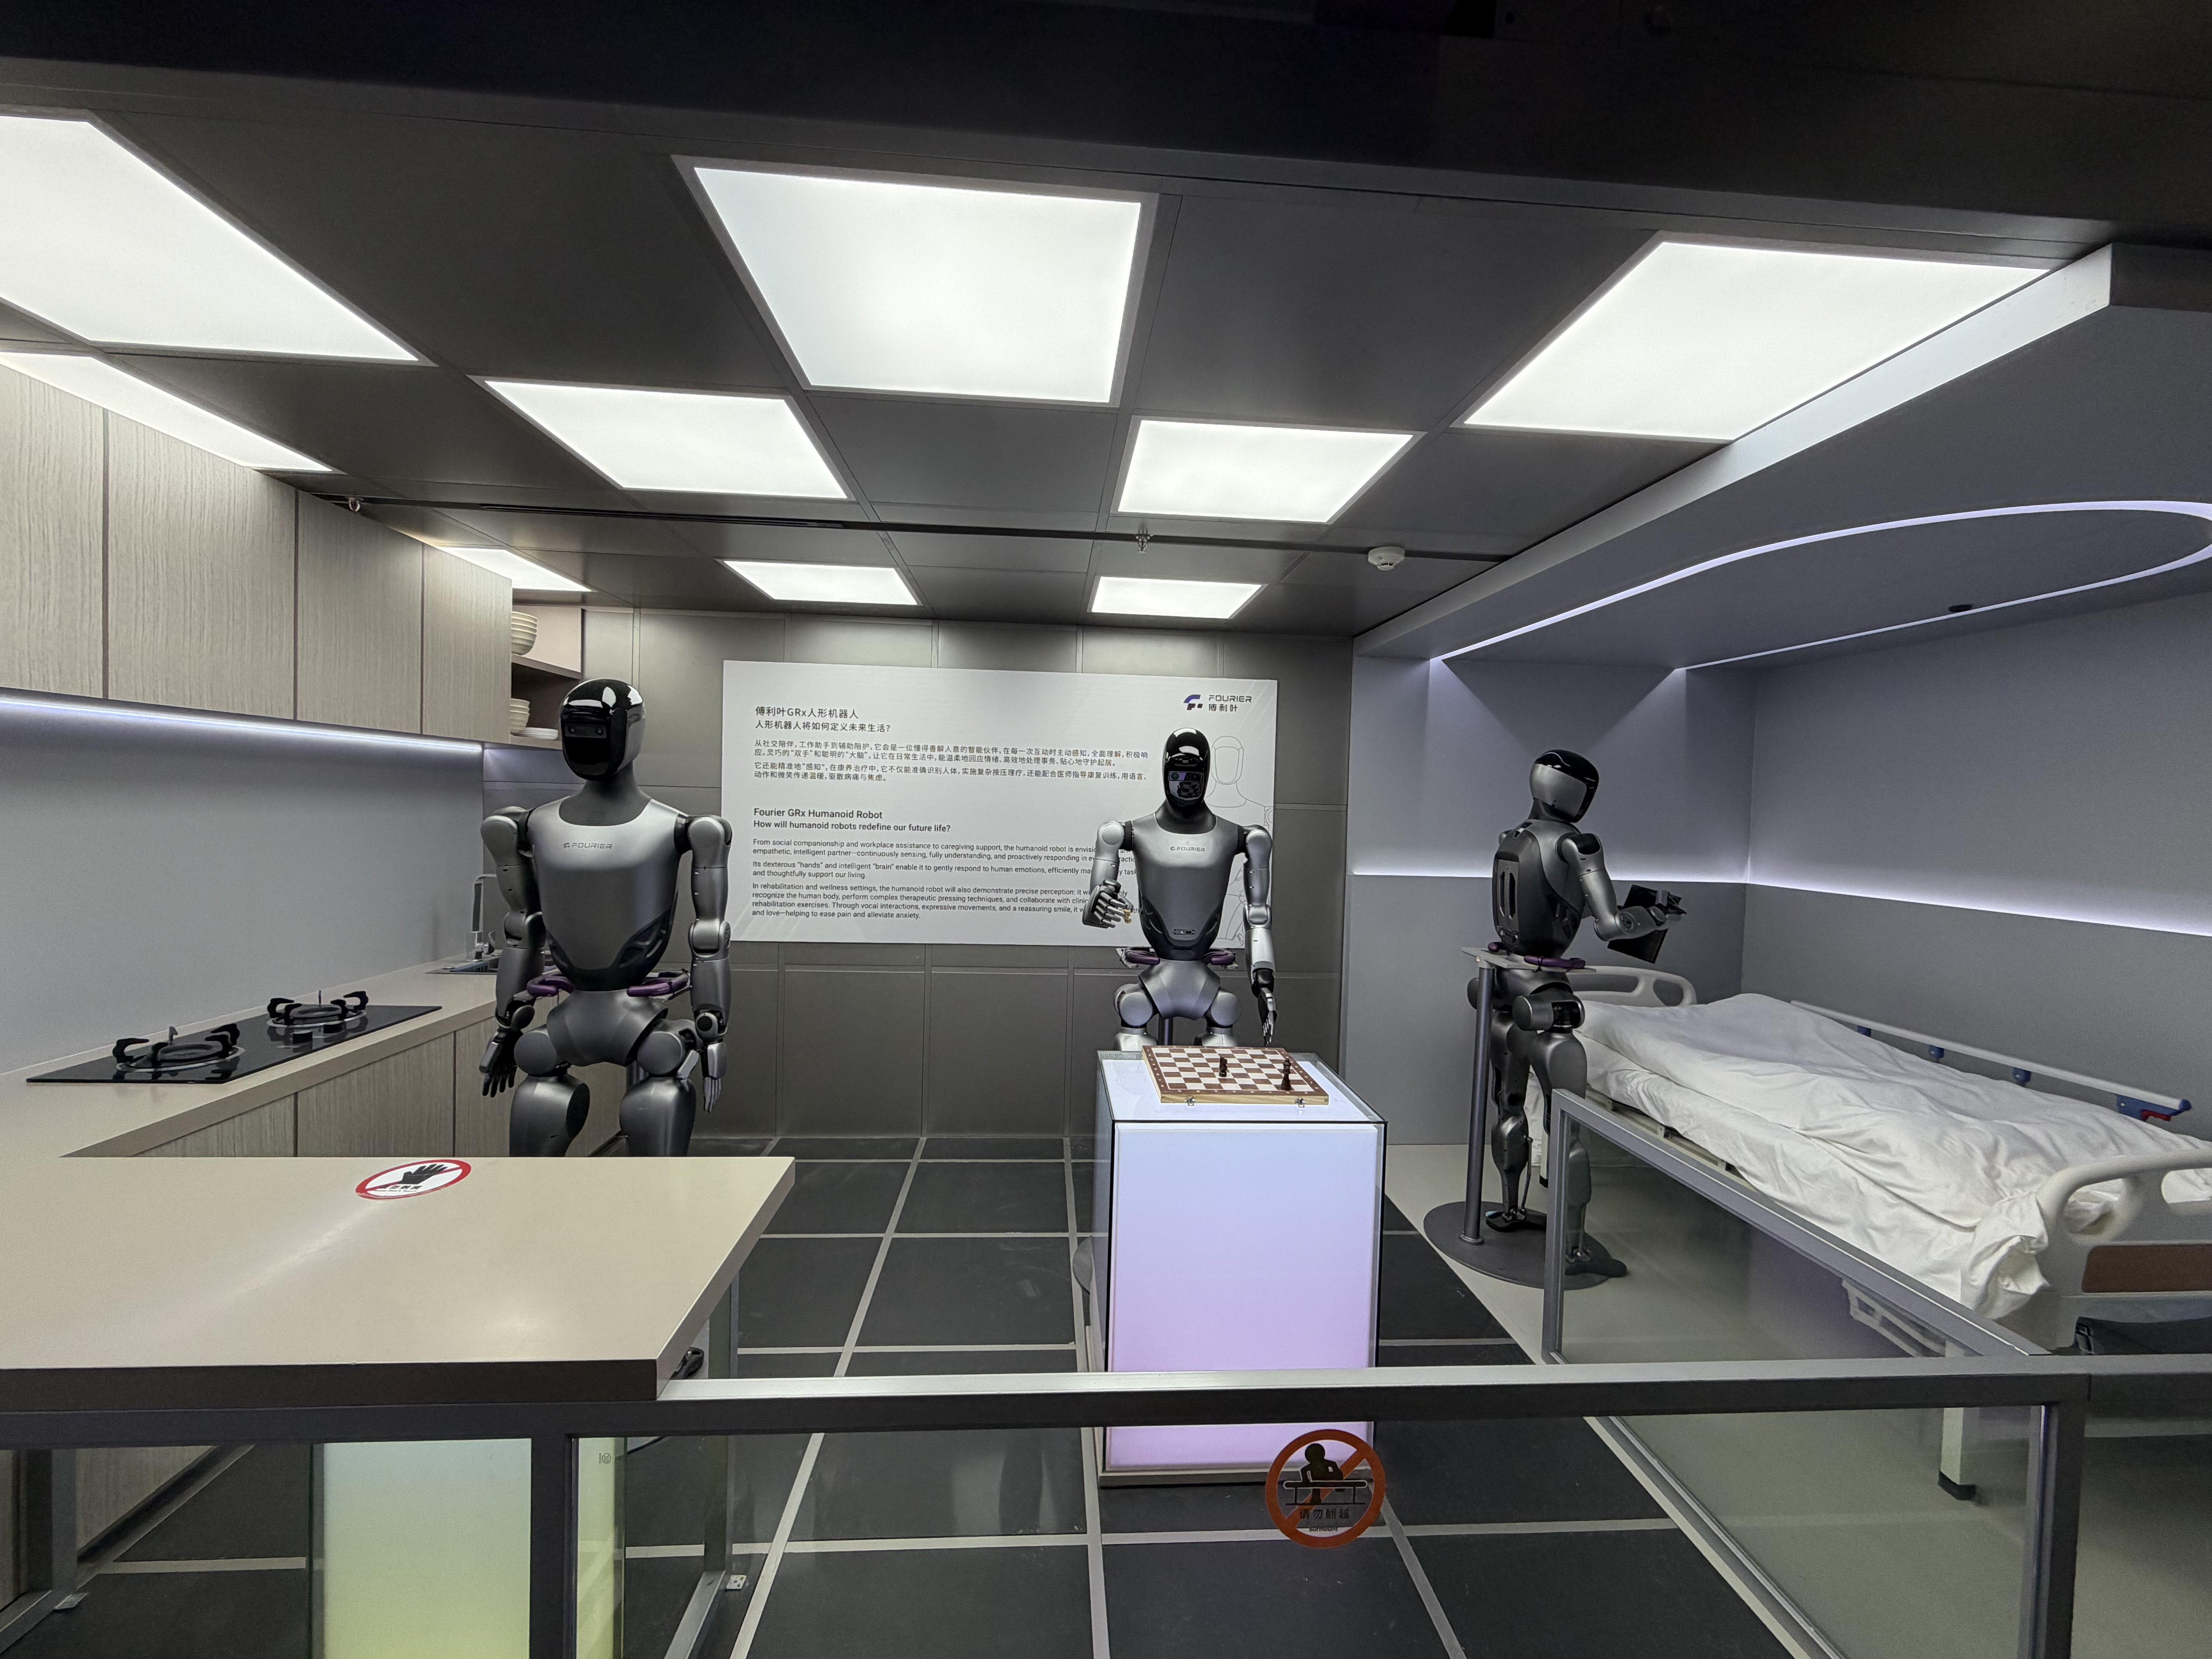
\includegraphics[width=0.62\linewidth]{field_trip/shanghai_science_technology_museum.jpg}
\end{center}
\noindent\textbf{Photograph caption:} Humanoid-robot exhibit at Shanghai Science and Technology Museum. Photograph by Yiqiao Liu (Mickey), September 4, 2026.

\noindent\textbf{Observation:} The photograph shows humanoid-robot figures, an exhibit panel, a chessboard, and a bed in a staged room. \textbf{Interpretation:} The exhibit prompted broader questions about how automated systems may coordinate decisions and responsibilities. It does not demonstrate free-riding, Nash equilibrium, or the current model's behavior.
